\chapter{Pathfinding}\label{ch:path}
Pathfinding is generally the process of finding a path from a starting point \emph{A}
to a destination \emph{B},
on a map.
Handling the map is explained in Chapter \ref{ch:map}.

There are different approaches to find the best path,
and different ideas what the best path is.

In the case of rescue, where time is very crucial to success,
the quickest path has to be considered best. \cite{Zipes2506}

In other applications 'best' could also mean shortest \emph{distance}, least expensive (toll roads),
most convenient or any number of other qualifiers.

Since our robot has approximately equal movement speed in all used directions,
the shortest time path can be approximated as the shortest distance path.

We chose to start implementing Dijkstra's shortest path algorithm,
since it is fairly simple to understand and can be used as a baseline for better,
more complex algorithms, like A*.

This chapter will explain the basics of different path finding approaches,
going more into detail on the ones we chose to implement for testing.

\section{Graphs}
The first step in most algorithms is to reduce the map to the necessary minimum.
After this reduction, the map only consists of \emph{nodes} and \emph{edges},
organized in a \emph{graph}.

An \emph{edge} connects two \emph{nodes} together and has a \emph{distance}.
In this integer is stored how much it costs to traverse along that \emph{edge},
measured in the metric that should get optimized (in our case distance and approximate time).

A \emph{node} has a \emph{name}, a \emph{cost to reach} and a reference to another \emph{node} \emph{parent}.
The name is used as an identifier,
\emph{cost to reach} sums the travelling costs to get here on the currently shortest path from the start.
\emph{Parent} refers to what \emph{node} is previous in that path.

There are two special \emph{nodes}, namely the starting \emph{node} and the finish \emph{node}.


\begin{figure}[h!tp]
    \centering
    \subfloat[Grid Graph]{
        \includegraphics[width=0.24\textwidth]{figures/path/graph_grid}
        \label{sub:grid}
    }
    \subfloat[Circular Graph]{
        \includegraphics[width=0.24\textwidth]{figures/path/graph_circular}
    }
    \subfloat[Tree Graph]{
    	\includegraphics[width=0.24\textwidth]{figures/path/graph_tree}
    }
  	\subfloat[Unstructured Graph]{
  		\includegraphics[width=0.24\textwidth]{figures/path/graph_unstructured}
	}
  	\caption{Different Representations of the same Graph}
  	\label{fig:graphs}
\end{figure}

Such a graph can be represented in any way,
as long as none of the described characteristics change.
Figure \ref{fig:graphs} shows four equivalent representations of the same graph.
We chose to omit any numbers for simplicity.

Since our prototype is running on a grid-like map,
the graph shown in Figure \ref{sub:grid} is our preferred representation,
since it is the easiest to relate to the real world for a human.
For the algorithm however, it doesn't matter.
\\\\
\section{Brute-Force}\label{sec:brute}
Brute-force is generally an algorithm,
that only relies on computational power,
instead of clever design.
For path-finding that would mean looking at all possible paths,
and evaluating which one is the shortest.
Brute-force algorithms can be implemented as a depth first search (DFS), or breadth first search (BFS).

\section{Flood Fill}\label{sec:fill}
Flood fill is looking at all neighbour \emph{nodes} from the start,
and looking at all their neighbours.
This process then gets repeated until the finish \emph{node} is reached.
Because the algorithm expands first in breadth,
this is a BFS-algorithm.

The name comes from visualising the algorithm,
which looks fairly similar to a liquid being spilled on a map.
%flood fill can be seen in Figure something later
\cite{Jaimini2017}

\section{Dijkstra}\label{sec:dijkstra}
Dijkstra's algorithm is a small improvement on the flood-fill algorithm explained earlier.
It takes into account the \emph{distances} between two \emph{nodes},
when deciding which \emph{node} to look at next.
Thus prioritising the easier to reach \emph{nodes}, when going to the next iteration.

This is done by storing all \emph{nodes} in a priority queue,
where they are sorted by their \emph{cost to reach}, in ascending order.

The \emph{cost to reach} gets calculated iteratively,
by adding the \emph{cost to reach} of the current \emph{node} together with the travel cost to its neighbour.
If that value is smaller than the \emph{cost to reach} currently stored in that neighbour,
the old value gets overwritten.
This process is shown stepwise in Figures \ref{sub:dijk1} through \ref{sub:dijk5}.
Those figures are also available in Appendix \ref{app:dijkstra}.\\
Observe how the value for the finish \emph{node} changes in almost every step,
until the finish \emph{node} is the current \emph{node}.

Every time the algorithm needs a new \emph{node} to evaluate its neighbours,
it takes the first element from that list.

\begin{figure}[h!]
	\begin{center}
		\foreach \dijk in {1,2,3,4,5}
		{
			\subfloat[\dijk. Step]{
				\includegraphics[width=0.175\textwidth]{figures/path/dijk_\dijk}
				\label{sub:dijk\dijk}
			}
		}
		\caption{Dijkstra's algorithm on a simple map}
		\label{fig:dijksteps}
	\end{center}
\end{figure}
% puts the table closer to the figure
\vspace{-0.75cm}
\begin{table}[h!]
\caption{Colour guide for Figure \ref{fig:dijksteps}}
\centering
\begin{tabular}{|l|p{4cm}|p{4cm}|}
	\hline%-------------------------------------------------------
	\multirow{2}{*}{Colour}	& \multicolumn{2}{c|}{Function}		\\
		 	& Nodes					&Edges						\\
	\hline%-------------------------------------------------------
	Red		&						&Used in current evaluation	\\
	\hline%-------------------------------------------------------
	Orange 	& Current Node			&							\\
	\hline%-------------------------------------------------------
	Green	& Evaluated Neighbour	&							\\
	\hline%-------------------------------------------------------
	White	& Not active yet		&							\\
	\hline%-------------------------------------------------------
	Black  &Shortest Path already found&Not used in current step\\
	\hline%-------------------------------------------------------
\end{tabular}
\end{table}

This approach has a huge benefit for maps,
where \emph{distances} between \emph{nodes} vary widely.
In our case \emph{distances} are one of two possibilities, either $1$ or $ \sqrt{2} $.
Thus making this effectively one implementation of a flood-fill search,
with the benefit, that only one addition needs to be done to implement A*,
which gets explained in Section \ref{sec:astar}.

\section{A*}\label{sec:astar}
A* uses Dijkstra's algorithm as a baseline,
but adds another value to each \emph{node}.
This value often gets called \emph{heuristic}.
Just like in Dijkstra, the \emph{cost to reach} gets calculated iteratively,
with the same iteration method.
But in A* there is also another 



\section{Pathfinding on a grid}
Pathfinding on a grid is slightly different to pathfinding on a regular map,
Because all \emph{nodes} tend to have the same amount of neighbours,
and all \emph{edges} have the same or similar costs.
Figure \ref{fig:graph_cost} shows the similarities between several connections on a grid-based graph.
because of this, the Dijkstra algorithm is losing its major advantage over a simple flood fill.
\begin{figure}[htp]
	\centering
	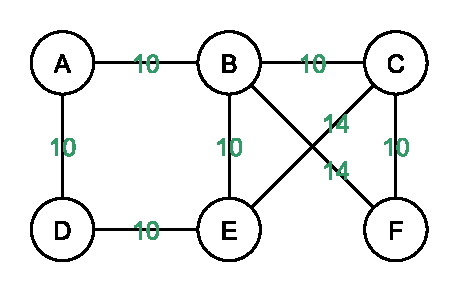
\includegraphics[width=0.24\textwidth]{figures/path/graph_values}
	\caption{3x3 grid with edge costs}
	\label{fig:graph_cost}
\end{figure}


\section{Our implementation}
\todo[inline]{does this belong into sec:map-handle?}
For our grid we chose to allow vertical, horizontal and diagonal movement,
giving us 8 possible directions to move in from every \emph{node}.
We decided to store those eight directions in one single byte,
with the least significant nibble (LSN) corresponding to the four main directions (N,E,S,W),
and the MSN corresponding to NE, SE, SW and NW.

\begin{center}
	\begin{tabular}{|*{8}{m{0.6cm}|}|l|}
		\hline
		N & E& S& W& NE& SE& SW& NW& byte\\
		\hline
		0 & 0 & 0 & 0 & 0 & 0 & 0 & 1 & 0x01\\
		0 & 0 & 0 & 0 & 0 & 0 & 1 & 0 & 0x02\\
		0 & 0 & 0 & 0 & 0 & 0 & 1 & 1 & 0x03\\
		0 & 0 & 0 & 0 & 1 & 1 & 1 & 0 & 0x0E\\
		\hline
		0 & 0 & 0 & 1 & 0 & 0 & 0 & 0 & 0x10\\
		0 & 0 & 1 & 0 & 0 & 0 & 0 & 0 & 0x20\\
		0 & 1 & 0 & 0 & 0 & 0 & 1 & 0 & 0x42\\
		1 & 1 & 1 & 1 & 1 & 1 & 1 & 1 & 0xFF\\
		\hline
	\end{tabular}
\end{center}

Just some random cites, to see how it works.
\cite{Madsen2010}, \cite{Oetiker2010} and \cite{Mittelbach2005}.
